\documentclass[german,english]{header}
%\usepackage{mathptmx}
\begin{document}
\selectlanguage{german}

\title{Agile Softwareentwicklung}
\subtitle{Einsatz und Werkzeuge im Open Source Umfeld}
\author{Tobias Dreher\and David Henn\and Mischa Vogt}
\institute{DHBW Stuttgart Campus Horb}

\maketitle
\begin{abstract}
Diese Seminararbeit beschäftigt sich mit agilen Methoden der Softwareentwicklung in Bezugnahme auf die Verwendung in Open-Source Projekten. Dabei werden die Entstehung der agilen Vorgehensweisen und die Methoden von \emph{Extreme Programming, Scrum} und \emph{Software Kanban} genauer erläutert. Danach wird die Verwendung agiler Vorgehensweisen bei größeren Open-Source Projekten wie beispielsweise \emph{TYPO3} genauer betrachtet. Zum Schluss werden mehrere Projektverwaltungswerkzeuge vorgestellt, die speziell auf die agile Entwicklung zugeschnitten sind, den Verwaltungsaufwand verringern und die Produktivität steigern sollen.
\end{abstract}

\section{Einleitung}
(Autor: Dreher)
\label{sec:einfuehrung}
Bis zur Jahrtausendwende waren \emph{V-Modell} und weitere Vorgehensmodelle, die auf Requirements Engineering aufbauen, vorherrschend in der Softwareentwicklung. Doch mit dem 1996 veröffentlichen \emph{Extreme Programming} änderte sich die Art der Planung, Entwicklung und Wartung von Software grundlegend. Dieser Prozess ist bis heute noch nicht abgeschlossen, jedoch gelten laut einer Studie von \emph{Forrester Research} agile Softwareentwicklungsprozesse inzwischen als ``Mainstream''. \cite{bib:ane}

Traditonelle Vorgehensmodelle gelten als sehr dokumentationslastig und schwergewichtig. Die Mitte der 90er Jahren entwickelten Vorgehensmodelle, die die Dokumentation eines Programms als zweitrangig ansahen, wurden daher als leichtgewichtig bezeichnet. Erst mit dem \emph{Manifesto for Agile Software Development} \cite{bib:manifest} entstand der Name ``Agile Vorgehensmodelle''. \cite{bib:eckstein} Das vor zehn Jahren veröffentliche Agile Manifest formuliert vier Wertvorstellungen, die für eine agiles Projekte gelten sollen:
\begin{enumerate}
	\item Individuen und Interaktionen mehr als Prozesse und Werkzeuge
	\item Funktionierende Software mehr als umfassende Dokumentation
	\item Zusammenarbeit mit dem Kunden mehr als Vertragsverhandlung
	\item Reagieren auf Veränderung mehr als das Befolgen eines Plans
\end{enumerate}

Des Weiteren stellten die ursprünglich 17 Unterzeichner des Manifests zwölf Grundprinzipen für agile Softwareentwicklung auf. \cite{bib:eckstein} Auf Grund deren Wichtigkeit in der agilen Softwareentwicklung seien diese hier aufgezählt:
\begin{enumerate}
	\item Unsere höchste Priorität ist es, den Kunden durch frühe und kontinuierliche Auslieferung wertvoller Software zufrieden zu stellen.
	\item Heisse Anforderungsänderungen selbst spät in der Entwicklung willkommen. Agile Prozesse nutzen Veränderungen zum Wettbewerbsvorteil des Kunden.
	\item Liefere funktionierende Software regelmäßig innerhalb weniger Wochen oder Monate und bevorzuge dabei die kürzere Zeitspanne.
	\item Fachexperten und Entwickler müssen während des Projektes täglich zusammenarbeiten.
	\item Errichte Projekte rund um motivierte Individuen. Gib ihnen das Umfeld und die Unterstützung, die sie benötigen und vertraue darauf, dass sie die Aufgabe erledigen.
	\item Die effizienteste und effektivste Methode, Informationen an und innerhalb eines Entwicklungsteam zu übermitteln, ist im Gespräch von Angesicht zu Angesicht.
	\item Funktionierende Software ist das wichtigste Fortschrittsmaß.
	\item Agile Prozesse fördern nachhaltige Entwicklung. Die Auftraggeber, Entwickler und Benutzer sollten ein gleichmäßiges Tempo auf unbegrenzte Zeit halten können.
	\item Ständiges Augenmerk auf technische Exzellenz und und gutes Design fördert Agilität.
	\item Einfachheit -- die Kunst, die Menge nicht getaner Arbeit zu maximieren -- ist essenziell.
	\item Die besten Architekturen, Anforderungen und Entwürfe entstehen durch selbstorganisierte Teams.
	\item In regelmäßigen Abständen reflektiert das Team, wie es effektiver werden kann und passt sein Verhalten entsprechend an.
\end{enumerate}
\section{Vorgehensmodelle}
Wie in Kapitel \ref{sec:einfuehrung} beschrieben, basieren alle Vorgehensmodelle auf wenigen klaren Regeln. Die bedeutendsten Modelle werden in diesem Kapitel genauer erläutert.

\subsection{Extreme Programming}
Extreme Programming (XP) ist eines der ältesten agilen Vorgehensmodelle und gibt Vorgaben für die Planung, das Management, das Quellcodedesign, das Testmanagement und die Programmierung eines Softwareprojekts. Dadurch wird XP sehr mächtig, aber auch anspruchsvoll für alle Beteiligten. \cite[S. 13]{bib:wolfRoock} \cite{bib:xp}

Einen Überblick über die Vorgehensweisen bei XP stellt die Abbildung \ref{fig:xppractices} dar. Der äußere Ring stellt die Planung da. Der mittlere Ring repräsentiert die Vorgehensweisen von Management und Design. Im inneren Ring sind die wichtigsten Punkte für das Testen und das Programmieren dargestellt.

\begin{figure}[h]
  \centering
  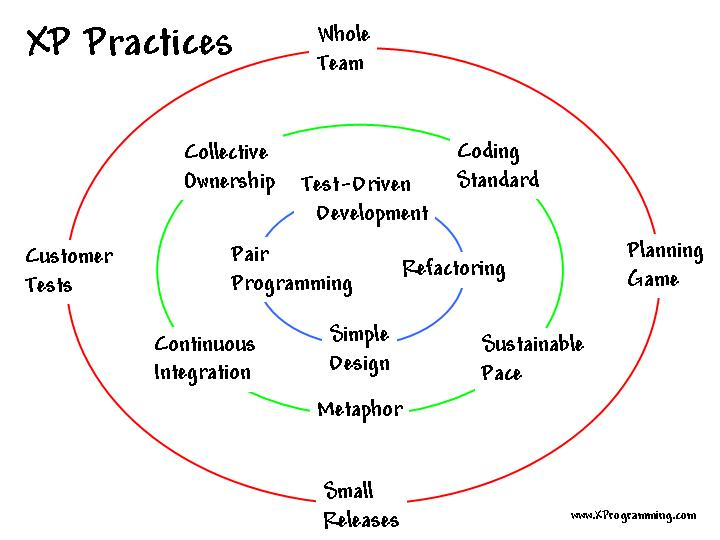
\includegraphics[width=0.8\textwidth]{images/xpCircles}
  \caption{Vorgehensweisen bei XP \cite{bib:xprogamming}}
  \label{fig:xppractices}
\end{figure}

\subsubsection{Planung}
Die Anforderungen an die Softwarelösung werden in sogenannten \emph{User Stories} festgehalten. Jede Story beschreibt eine Funktion, die der Kunde möchte. Eine solche User Story könnte wie folgt lauten:
\begin{quote}
Anzeige einer Druckvorschau beim Auswählen der Druckfunktion
\end{quote}
Danach wird ein Release-Plan erstellt. In der Regel werden alle drei Monate Releases veröffentlicht. Bei der Erstellung des Plans legen die Entwickler fest, welche User Story in welchem Release implementiert werden soll. Der Zeitraum zwischen zwei Releases wird wiederum in ein- bis drei-wöchige Iterationen unterteilt. Zu Beginn jeder Iteration wählt der Kunde, die für ihn wichtigsten User Stories aus. Die Entwickler entwerfen, implementieren und testen die ausgewählten Stories innerhalb der Iteration. Am Ende jeder Iteration muss das Programm lauffähig sein, auch wenn noch wichtige Funktionen fehlen.

\subsubsection{Management}
Auch für das Management eines Softwareprojekts sind bei XP klare Regeln definiert. Täglich gibt es ein Meeting, bei dem jeder Entwickler kurz sagt, was er am Vortag getan hat, was er heute tun wird und welche Probleme er sieht. Eine weitere wichtige Regel ist, dass ein Entwickler nicht länger arbeiten darf, als er auf unbefristete Zeit leisten kann. Normalerweise sind dies acht Stunden pro Tag. Überstunden sind nicht gern gesehen. Des Weiteren soll jeder Entwickler in den gesamten Prozess eingebunden sein und immer über den Gesamtstand des Projektes informiert sein. Außerdem sollen Entwickler immer wieder mit anderen Aufgaben betraut werden. Damit soll vermieden werden, dass sie den Anschluss zum technologischen Geschehen verlieren. Aus dem selben Grund soll den Entwicklern auch genügend Freiraum gegeben werden, um auch während eines Projekts sich mit technischen Neuerungen zu befassen.

\subsubsection{Quellcodedesign}
Da im Gegensatz zu traditionellen Vorgehensmodellen die endgültige Architektur der Softwarelösung während der Programmierung noch nicht klar ist, sind beim Design einige Regeln zu beachten. Die wichtigste ist hier die Einfachheit. Der Quellcode ist so einfach wie möglich zu halten. Es sollen keine unnötigen Funktionen implementiert werden und es ist so zu programmieren, dass jeder aus dem Team den Quellcode verstehen kann. Des Weiteren soll immer wenn es sinnvoll ist, refactort werden.

\subsubsection{Testmanagement}
Bei Extreme Programming wird testgetrieben entwickelt. Das heißt, es werden zuerst die Unit-Tests einer Funktion geschrieben. Erst danach darf die Funktion selbst geschrieben. Diese Art der Programmierung zwingt den Programmierer zu einer genaueren Überlegung, was die Funktion erledigen soll und welche Grenzfälle dabei auftreten können. Und dabei stellt das \emph{Test First} genannte Prinzip gleichzeitig sicher, dass es eine komplette Testabdeckung gibt. Die Unit-Tests werden mehrmals täglich ausgeführt. Zur weiteren Verbesserung der Qualität werden die Änderungen der Entwickler mehrfach am Tag in die gemeinsame Quellcodebasis integriert. Dieser Integrationstest stellt sicher, dass die einzelnen Teilkomponenten korrekt miteinander arbeiten. Noch eine Stufe abstrakter ist der \emph{Acceptance Test}. Dies ist ein Black-Box-Test, der nach jeder Iteration vom Kunde durchgeführt wird. Jeder Fehler, der vom Kunde gemeldet wird, muss mit einem Unit-Test abgedeckt werden um ihn zukünftig zu vermeiden.

\subsubsection{Programmierung}
Die auffälligste Unterscheidung von XP zu traditionellen Vorgehensmodellen ist das \emph{Pair Programming}. Es sitzen immer zwei Entwickler vor einem Rechner und einer Tastatur und programmieren gemeinsam. Dabei wechseln sie sich regelmäßig beim Schreiben des Codes ab. Dies soll bei geringem Zeitverlust eine starke Qualitätssteigerung mit sich bringen. Weniger auffällig, aber trotzdem wichtig ist die Regel, dass jeder Entwickler das Recht hat jede Codezeile des Projektes zu ändern. Das heißt, wenn ihm Fehler oder Unstimmigkeiten auffallen, kann er diese gleich beheben.

\subsection{Scrum}
\label{ch:scrum}
Laut einer Studie von 2010 von \emph{Forrester Research} ist Scrum die verbreitetste agile Methode. So verwendeten ca. 11 \% der befragten IT-Fach\-kräfte das wohl bekannteste agile Vorgehensmodell. \cite{bib:ane} Scrum bietet deutlich weniger Regeln als Extreme Programming und gilt somit als verhältnismäßig leicht einzusetzen. 

\subsubsection{Rollenverteilung}
Im Zentrum von Scrum steht ein hochmotiviertes und selbstgesteuertes Entwicklerteam. Die Rollenverteilung von klassischen Vorgehensmodellen wird grundlegend verändert. Der Produktmanager wird zum Product Owner. Der Teamleiter wird zum Scrum Master. Und das Team, zu dem alle Entwickler gehören, bekommt deutlich mehr Verantwortung.

\begin{description}
\item Product Owner\\
Er bringt die Produktvision mit sich und ist verantwortlich für das Produkt. Dabei definiert er die Anforderungen, priorisiert sie und kontrolliert die Ergebnisse. Zusätzlich behält er das Budget und die Wirtschaftlichkeit im Blick. Wichtig: Der Product Owner gibt dem Team keine Zeitvorgaben.

\item Scrum Master\\
Der Scrum Master sorgt für die Einhaltung des Entwicklungsprozesses und den Scrum-Regeln. Hierzu schützt er das Team auch vor Störungen von außen und beseitigt organisatorische Probleme. Wichtig: Der Scrum Master vergibt keine Aufgaben.

\item Team\\
Das Team steht im Mittelpunkt des Entwicklungsprozesses. Es entscheidet selbst wann es welche Aufgaben erledigt. Verantwortung übernimmt das Team für das Zeit-, Qualitäts- und Dokumentationsmanagement.
\end{description}

\subsubsection{Prozess}
Die Abbildung \ref{fig:scrum} stellt das Vorgehen bei Scrum dar. Zu Beginn des Projekts stellt der Product Owner das \emph{Product Backlog} auf, in dem die Anforderungen des Produkts mit User Stories beschrieben werden. Das Product Backlog kann jederzeit vom Product Owner mit weiteren Anforderungen erweitert werden. Jede Anforderung bekommt vom Product Owner eine Priorität, die sich auch im Laufe des Projekts verändern kann. Das priorisierte Product Backlog stellt der Product Owner im \emph{Sprint Planning Meeting} dem Team vor. Beim Sprint Planning Meeting wählt das Team so viele User Stories aus dem Product Backlog aus, wie es denkt während der nächsten Iteration (\emph{Sprint} abarbeiten zu können. Die User Stories teilt das Team in einzelne Aufgaben auf und hält sie im \emph{Sprint Backlog} fest. Das Sprint Backlog darf während einer Iteration nicht verändert werden.

\begin{figure}[h]
  \centering
  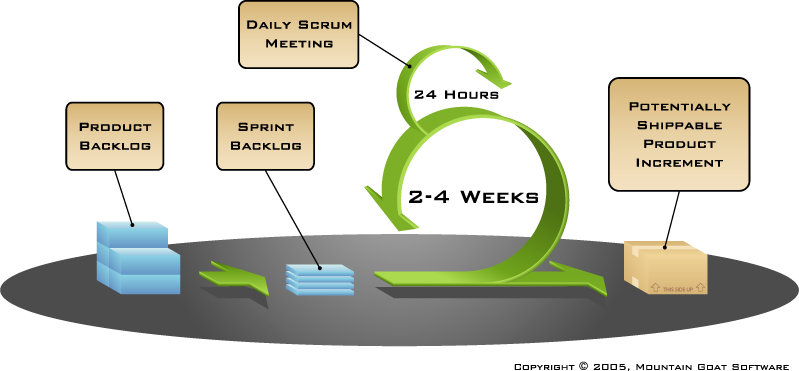
\includegraphics[width=1\textwidth]{images/scrum}
  \caption{Prozessüberblick bei Scrum \cite{bib:mountaingoat}}
  \label{fig:scrum}
\end{figure}

Nach dem Meeting beginnt der Sprint. Ein Sprint stellt eine Iteration von zwei bis vier Wochen dar und wird immer wieder durchlaufen. Während des Sprints findet täglich ein \emph{Daily Scrum Meeting} statt an dem das Team und der Scrum Master teilnehmen. Dieses ist gleich aufgebaut wie das tägliche Meeting beim Extreme Programming. Die Dauer des Meetings legt der Scrum Master in der Regel auf 15 Minuten fest und hält dies auch ein. Jeder Teilnehmer bespricht kurz die folgenden drei Dinge:
\begin{itemize}
  \item Was habe ich gestern gemacht? 
  \item Was steht heute auf dem Plan? 
  \item Und welche Probleme habe oder sehe ich?
\end{itemize}
Im Sprint Backlog wird der tägliche Fortschritt festgehalten. Dadurch entsteht ein immer aktuelles Burn-Down Diagramm (Abbildung \ref{fig:burndown}), das den Fortschritt des Sprints übersichtlich darstellt. 

\begin{figure}[h]
  \centering
  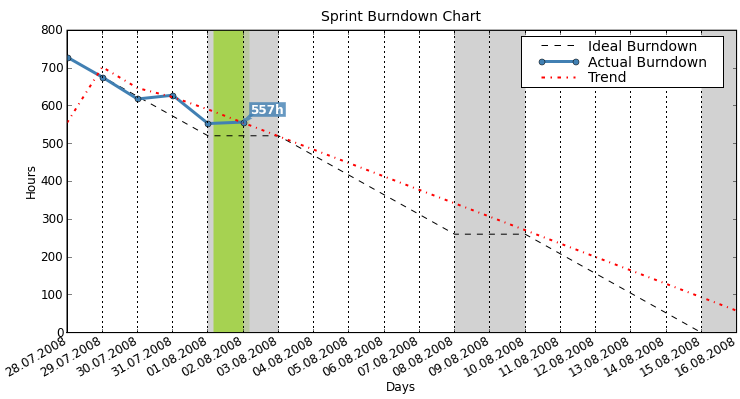
\includegraphics[width=1\textwidth]{images/burndown}
  \caption{Burn-Down Diagramm eines Sprints \cite{bib:agilo}}
  \label{fig:burndown}
\end{figure}

Am Ende des Sprints muss eine lauffähige Version des Programms verfügbar sein, die dem Product Owner im \emph{Sprint Review Meeting} präsentiert wird. Zusätzlich gibt es noch das \emph{Sprint Retrospective Meeting}, an dem über den vergangen Sprint reflektiert wird um über Veränderungen eine Verbesserung des Prozesses zu erzielen.

\subsubsection{Scrum Anti-Pattern}
Marion Eickmann schreibt, dass Scrum nur dann funktioniert, wenn auch alle Beteiligten sich an die Regeln halten: ``Alle Beteiligten müssen sich an das neue Vorgehen gewöhnen und sind unsicher was zu tun ist, wenn Unerwartetes geschieht. Solche Schwierigkeiten führen häufig dazu, `bekannte' Mechanismen `nur für den Fall' anzuwenden, statt das Problem nach Scrum-Art zu lösen.'' \cite[S. 84]{bib:ix2010}. So führt sie in ihrem Artikel mehrere bekannte Scrum Anti-Pattern auf, die es gilt zu vermeiden. Die wichtigsten seien hier aufgezählt:
\begin{itemize}
  \item Der Scrum Master weist Tasks zu und zerstört so das sich selbst steuernde und organisierende Team
  \item Der Sprint wird von außen gestört. Es werden neue Aufgaben eingefügt oder Änderungen an den gewählten (committed) User Stories vorgenommen.
  \item Es finden keine Review Meetings statt
  \item Es findet keine Retrospective statt
  \item Es gibt keine regelmäßigen Daily Standup Meetings
  \item Der Product Owner hat keine ausreichende Kompetenz und nimmt seine Rolle nicht war
  \item Meetings sind nicht Time-Boxed
  \item Statt Funktionen werden Aktivitäten erfasst
\end{itemize} 

\subsubsection{Verknüpfung mit anderen Methoden}
Da Scrum lediglich Vorgaben für die Planung und das Management eines Softwareprojekts macht, wird es oftmals mit anderen Vorgehensmodellen kombiniert. So können zum Beispiel die Punkte Quellcodedesign, Testmanagement und Programmierung von Extreme Programming übernommen werden. Das kombinierte Vorgehensmodell hat zwar viele Regeln, die es gilt einzuhalten, aber deckt den kompletten Softwareentwicklungsprozess ab.

\subsection{Software Kanban}
Software Kanban ist die jüngste der hier vorgestellten Methoden und unterscheidet sich auch stark ihnen. So gibt Software Kanban nicht vor wie man ein Projekt durchführt, sondern lediglich wie man den Prozess von einer klassischen Vorgehensweise in eine Agile umwandelt (\emph{Change Management Methode}). \cite[S. 14]{bib:wolfRoock} Dabei wird versucht den Entwicklungsprozess Schritt für Schritt zu verbessern, statt einen radikalen Schnitt wie bei Scrum oder XP zu wagen. Dies minimiert die Widerstände der einzelnen Beteiligten gegenüber großen Veränderungen. \cite{bib:ix2011}

\subsubsection{Grundprinzipien}
David J. Anderson \cite{bib:anderson}, der Erfinder von Software Kanban, definiert drei Grundprinzipien für die Methode:
\begin{itemize}
  \item Beginne dort, wo du dich im Moment befindest
  \item Komme mit den anderen überein, dass inkrementelle, evolutionäre Veränderungen angestrebt werden
  \item Respektiere den bestehenden Prozess sowie die existierenden Rollen, Verantwortlichkeiten und Berufsbezeichnungen
\end{itemize}

Durch das erste Grundprinzip entstehen viele verschiedene Implementierungen der Methode. So kann Software Kanban an ein bestehendes Wasserfallmodell gekoppelt werden oder auch eine bestehende Implementierung des V-Modells langsam verändern und verbessern.

Des Weiteren definiert Anderson fünf Kerneigenschaften von Software Kanban, die im folgenden näher erläutert werden.

\subsubsection{Visualisierungen}
Als erster Schritt in Software Kanban wird der aktuelle Entwicklungsprozess visualisiert. Es bietet sich ein Whiteboard mit den einzelnen Prozessschritten als Spalten dargestellt an. Ein solches Whiteboard ist in Abbildung \ref{fig:kanbanBoard} dargestellt. Typische Prozessschritte sind zum Beispiel:
\begin{itemize}
  \item Idee/Bestellung (Backlog)
  \item Eingeplant
  \item Entwicklung
  \item Test
  \item Auslieferung
  \item Produktiv
\end{itemize}

Zu jeder Spalte sind eine oder mehrere Personen zugeordnet. Wenn es bei der Vorgängermethode zum Beispiel auch Softwarearchitekten gab, muss eine Spalte \emph{Design} hinzugefügt werden. Die Spalten \emph{Entwicklung} und \emph{Test} werden nochmals unterteilt in \emph{laufend} und \emph{erledigt}. 

\begin{figure}[h]
  \centering
  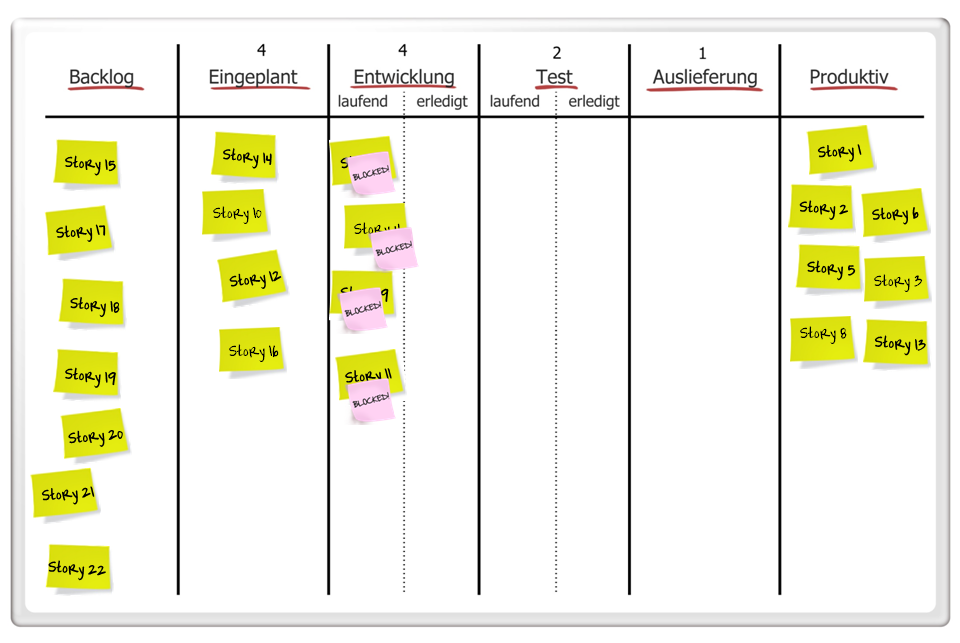
\includegraphics[width=1\textwidth]{images/kanbanBoard}
  \caption{Visualisierung eines Entwicklungsprozesses in Software Kanban \cite{bib:roock}}
  \label{fig:kanbanBoard}
\end{figure}

Die einzelnen Anforderungen (\emph{Ticket}) an das Softwareprodukt werden auf Haftnotizen oder Karteikarten geschrieben, mit einer Priorität versehen und in die Spalte \emph{Backlog} geheftet. Jede Anforderung durchläuft nun den gesamten Prozess, wobei immer notiert wird, wann die Anforderung in welcher Spalte aufgenommen wurde.

Ein kleiner Bruch mit der Vorgängermethode stellt nun das \emph{Pull-Prinzip} dar. Wer eine Aufgabe erledigt hat, darf sich in der Vorgängerspalte eine neue Anforderung nehmen und abarbeiten. Eine Überbelastung der Beteiligten wird damit vermindert, da jeder selbst entscheidet wie viel Arbeit er auf sich nimmt und in welcher Geschwindigkeit er diese bewältigt.

\subsubsection{Begrenzungen}
Für jede Spalte wird nun ein \emph{Work in Progress-Limit} (\emph{WiP-Limit}) festgelegt. Es bestimmt wie viel Tickets pro Prozessschritt maximal gleichzeitig bearbeitet werden dürfen. Dadurch minimieren sich Zeitverlust und Flüchtigkeitsfehler durch häufige Kontextwechsel. Außerdem werden Engpässe schneller sichtbar. Wenn zum Beispiel die Testabteilung ständig am Limit arbeitet, sollten hier eventuell mehr Personen eingesetzt werden.
Die WiP-Limits werden wie in Abbildung \ref{fig:kanbanBoard} zu jeder Spalte geschrieben.

\subsubsection{Messungen}
Eine weitere Kerneigenschaft von Software Kanban ist die ständige Erstellung von Metriken. Hierbei sind zwei Messungen besonders wichtig:
\begin{description}
  \item Lead Time\\ Durchlaufzeit einer Anforderung vom Backlog bis zur Auslieferung
  \item Cycle Time\\ Reine Entwicklungszeit ohne Wartezeiten
\end{description}
Weitere Messungen sind unter anderem \emph{Durchsatz}, \emph{Fehlerrate} und \emph{Termintreue}. Durch die Darstellung der Metriken werden Engpässe und Verbesserungsmöglichkeiten sichtbar. Auch die Tickets werden überwacht und z.B. als Cumulative Flow Chart (Abbildung \ref{fig:kanbanChart}) dargestellt.

\begin{figure}[h]
  \centering
  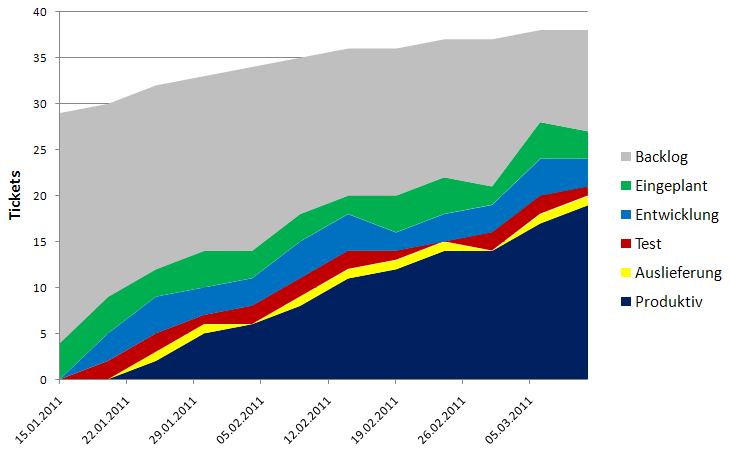
\includegraphics[width=1\textwidth]{images/kanbanChart}
  \caption{Cumulative Flow Chart der Tickets}
  \label{fig:kanbanChart}
\end{figure}

\subsubsection{Prozessregeln}
Um die Vorgehensweise für alle Beteiligten transparent darzustellen werden alle Regeln festgehalten. Es bietet sich an alle Prozessregeln direkt neben dem Whiteboard anzubringen. Beispiele für solche Regeln sind:
\begin{itemize}
  \item Wodurch kommen Tickets in das Backlog?
  \item In welcher Reihenfolge werden Tickets abgearbeitet?
  \item Wann dürfen WiP-Limits gebrochen werden
  \item Wie werden Bugs in dem Prozess behandelt?
\end{itemize}

\subsubsection{Verbesserungen}
Die fünfte Kerneigenschaft von Software-Kanban ist die kontinuierliche Verbesserung. Hierzu können nach und nach weitere Merkmale von anderen agilen Vorgehensmodellen wie Scrum und XP übernommen werden. So kann ein tägliches Stand-Up-Meeting die Kommunikation erhöhen. Pair Programming erhöht die Qualität. Test First verbessert ebenfalls die Qualität. 

Wichtig bei der Einführung der neuen Merkmale ist die Akzeptanz bei allen Beteiligten. Wenn der Verbesserungsprozess zu schnell durchgeführt wird, werden einige Beteiligte sich gegen die Veränderungen wehren und den gesamten Prozess stören. Ob eine Veränderung auch eine Verbesserung der Situation bedeutet kann mit den erstellten Metriken überprüft werden. Im Notfall sollte die Veränderung auch wieder rückgängig gemacht werden können.
\section{Agile Methoden und Open Source}
(Autor: Henn)\\

Agile Methoden sind zur Zeit voll im Trend. Die Fachzeitschriften sind voll davon und in Firmen
werden agile Vorgehensweisen immer häufiger umgesetzt. Doch wie sieht die Situation in Open Source
Projekten mit ganz anderen Umständen und Herausforderungen aus?

In diesem Abschnitt wird ein Blick in die Open Source Welt geworfen und
analysiert, inwiefern agile Techniken eingesetzt werden. Im Anschluss werden
Chancen und Probleme bei der Verwendung eines agilen Modells im Open Source
Bereich dargestellt.


\subsection{Open Source Projekte}
Bei der Recherche viel auf, dass es gar nicht so leicht ist, Open Source
Projekte zu finden, die von sich selbst behaupten, sie würden nach agilen
Vorgehensmodellen vorgehen. Allerdings finden sich auch in normalen Projekten
Techniken, die eindeutig aus der agilen Softwareentwicklung kommen. Im Folgenden
sollen einige Projekte als Stellvertreter für die verschiedenen Stufen der
Adaption mit Blick auf die Umsetzung agiler Techniken und Prinzipien betrachtet werden.

\subsubsection{TYPO3}
Die Entwickler des Open Source Content Management Systems TYPO3 haben sich dazu
entschieden, ihre nächste Version 5 (Phoenix) vollständig nach dem Scrum Vorgehensmodell zu
entwickeln. Anhand dieses Beispiels soll gezeigt werden, wie es möglich ist,
ein solches Vorgehensmodell im Open Source Bereich vollständig umzusetzen und
was es für Bedingungen gibt, damit dies erfolgreich geschehen kann.
\begin{figure}[h]
	\centering
	
\includegraphics[width=1\textwidth]{images/typo3_Phoenix_logo.jpg}
	\caption{Logo TYPO3 5.0 Phoenix}
	\label{Logo-Phoenix}
\end{figure}

Ein Sprint dauert beim TYPO3 Phoenix Team 4 Wochen. Innerhalb dieses Sprints finden tägliche
Meetings statt und am Ende eines Sprints muss eine lauffähige Version bereit stehen. Abbildung 
\ref{magic-cycle} visualisiert diesen Zyklus. User Stories aus dem Product Backlog werden für
diesen Sprint ausgesucht und in einem Sprint Backlog festgehalten. Diese Stories werden dann
innerhalb der 2-4 Wochen implementiert.
\begin{figure}[h]
	\centering
	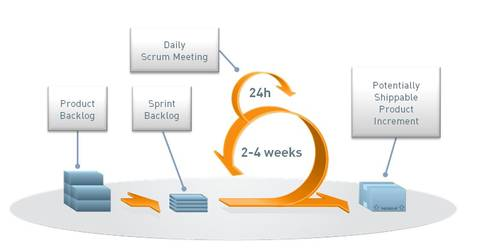
\includegraphics[width=1\textwidth]{images/typo3-magic-cycle.jpg}
	\caption{Magic Cycle - TYPO3 Scrum Implementierung}
	\label{magic-cycle}
\end{figure}


Als Product-Owner, der in Firmen in der Regel aus einer Person besteht, wurde für TYPO3
ebenfalls ein kleines Team bestehend aus drei Personen eingerichtet. Dies erscheint sinnvoll, da es
sich bei TYPO3 ja um eine Gemeinschaftsentwicklung handelt. Eine einzelne Person als Product-Owner
würde dem Community Gedanken entgegen wirken und  wäre darüber hinaus Person wahrscheinlich auch
noch überlastet, wenn sie plant, diese Aufgabe in ihrer Freizeit auszufüllen. Diese drei
Personen diskutieren über die Features, die innerhalb eines Sprints implementiert werden sollen
und priorisieren diese.
\newline Die Rolle des Scrum-Masters wird wiederum nur von einer Person besetzt. Auch dies ergibt
durchaus Sinn, da sich zwei Scrum-Master, oder sogar ein Team von Scrum-Masters eher gegenseitig bei
der Leitung von Gesprächen behindern würde.
\newline Das eigentliche Scrum-Team für die TYPO3 Entwicklung besteht aus 19 Entwicklern. Die alle
miteinander in Kontakt stehen und koordiniert werden müssen. Entscheidend für den Erfolg von Scrum
ist daher das Internet. Es bietet vielfältige Möglichkeiten, miteinander zu kommunizieren und große
räumliche Entfernungen zu überbrücken. So kommuniziert das Team:
\begin{itemize}
\item Sprint-Planung, Review und Retrospektive werden durch Meetings im Internet durchgeführt.
\item Es steht ein Jabber Chatroom bereit, in dem sich das Team kurzfristig abstimmen kann und
Fragen während der Entwicklung geklärt werden.
\item jeden Tag findet um 17:00 Uhr das Daily Scrum Meeting mittels Webex oder Skype statt. Danach
wird das Protokoll der Sitzung über die Mailing Liste verschickt, damit alle, die nicht teilnehmen
konnten, trotzdem auf dem neusten Stand sind.
\item Das Sprint-Backlog wird ebenfalls im Internet unter forge.typo3.org gepflegt.
\item TYPO3 Veranstaltungen werden so oft, wie möglich genutzt um persönlich miteinander sprechen zu
können
\item Nach jedem Sprint wird das Ergebnis sowohl als Nachricht, als auch als laufende
Demo-Installation bekanntgegeben
\end{itemize}
\begin{figure}[h]
	\centering
	\fbox{
		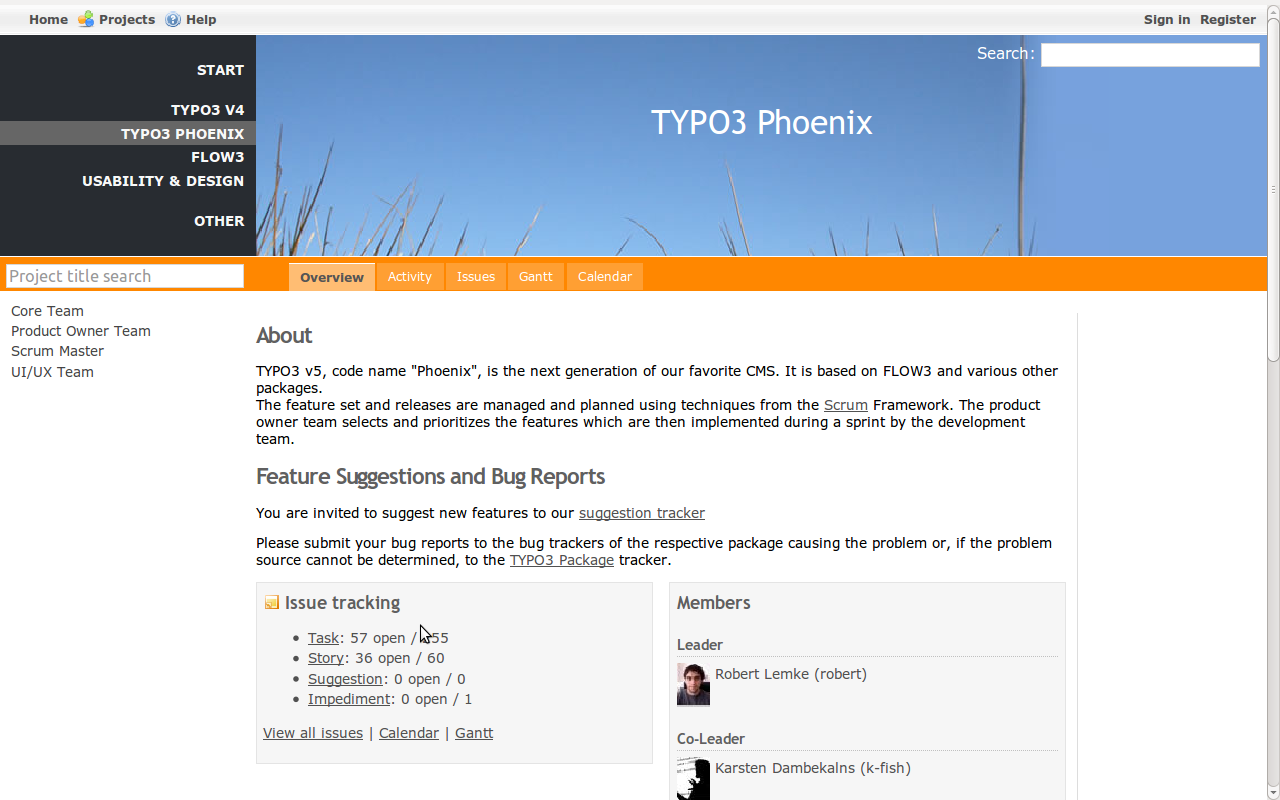
\includegraphics[width=1\textwidth]{images/forge-typo3-org.png}
	}
	\caption{forge.typo3.org}
	\label{forge}
\end{figure}
Der gesamte Fortschritt sowie die offizielle Dokumentation und Kommunikation wird über
die Web-Plattform forge.typo3.org dargestellt. Auf diese Weise ist der Entwicklungsprozess sehr
transparent und für die Community einsehbar. Dadurch verliert die Entwicklung nicht an Akzeptanz und
die freiwilligen Committer wissen, was gerade benötigt wird.

Auf der Website des Phoenix Teams wurden mehrere Bereiche eingerichtet:
\begin{description}
\item [Core Team] Hier befinden sich alle Informationen, die das Entwicklungs-Team zur Koordination
benötigt. der Bereich beinhaltet
\begin{itemize}
\item eine Übersicht mit Link zum Issue-Tracker und einer Liste der Team Mitglieder
\item Eine Auflistung aller bisher ausgeführten Aktivitäten, wie Wiki Änderungen, oder auch
Änderungen am Quellcode
\item Eine Roadmap für den aktuellen Sprint, mit Auflistung aller in diesem Sprint zu erledigenden
User Stories und den dazugehörigen Tasks
\item den Issue Tracker
\item das Sprint, sowie das Product Backlog
\item ein Gantt Chart
\item ein Kalender
\item  ein Wiki
\item das Repository mit dem Quellcode
\end{itemize}
Das Wiki beinhaltet alle wichtigen Informationen für Entwickler, sowie teilweise Erklärungen zum
Scrum Prozess und Richtlinien.  So findet sich dort zum Beispiel die Erklärung, was es mit der
''Definition of Done``  auf sich hat, die bei Scrum ein wichtiges Artefakt darstellt.
\item [Product Owner Team] Für das Product Owner Team gibt es ebenfalls wie beim Core Team eine
Übersicht mit den Mitgliedern, sowie eine kurze Beschreibung der Gründe, sich für ein Teams als
Product Owner zu entscheiden. Es finden sich ebenso Übersichten über Aktivitäten, Issues und
Termine. Außerdem wird ebenfalls ein Wiki gepflegt. Dieses Wiki behandelt  allerdings viel
stärker den Scrum Entwicklungsprozess, als das Wiki des Core Teams. So ist hier der eigentliche
Entwicklungsprozess für TYPO3 Phoenix beschrieben, sowie für alle, die Scrum noch nicht so intuitiv
leben ein kleines Cheat Sheet hinterlegt, das den Scrum Prozess nochmal auf einer Seite
übersichtlich zusammenfasst. Ebenso findet sich hier eine Liste mit Benutzerrollen für TYPO3. Im
Anschluss daran sind die Protokolle der einzelnen Scrum Meetings hinterlegt.
\item [Scrum Master] im Bereich des Scrum Masters gibt es lediglich eine Übersicht, einen Bereich
in dem die Aktivitäten aufgelistet werden, sowie Issue Tracker, Gantt Chart und ein Kalender. Da
die Rolle des Scrum Masters nur mit einer Person besetzt ist, muss hier auch nicht mehr Inhalt
bereit stehen.
\item [UI/UX Team] dieses Team beschäftigt sich mit dem User Interface, sowie der User Experience.
Es finden sich die Übersichten, über Issues und Aktivitäten, wie in den anderen Bereichen. 
\end{description}

Die TYPO3 Entwickler haben es geschafft, den gesamten Scrum Prozess mit minimalen Anpassungen
für ihr Projekt zu Adaptieren. Von entscheidendem Vorteil für die TYPO3 Entwickler, ist die
Tatsache, dass sie alle aus Deutschland kommen. So ist es deutlich einfacher, einen Termin, der auf
17:00 Uhr angesetzt ist, wahrzunehmen. Eine solche regelmäßige zeitliche Abstimmung würde bei
Entwicklern, die über die ganze Welt verstreut sind nicht funktionieren. Außerdem ist es so für die
Projektteilnehmer leichter, zu den TYPO3 Veranstaltungen zu fahren, da diese ebenfalls hauptsächlich
in Deutschland stattfinden. Auch hier wäre es für einen weit verstreutes Entwicklerteam
auch finanziell nicht möglich, sich so oft persönlich zu sehen. Ein weiterer Faktor ist sicherlich
die Größe des Projektteams. Bei nur 17 Mitgliedern ist es leichter möglich, alle über das Internet
zu koordinieren und dafür zu sorgen, dass auch wirklich alle gerade aktiv am Projekt
teilnehmen können.



\subsection{Vorteile agiler Methoden in Open Source Projekten}
  - Motivation von Entwicklern und Community\\
  - Rasches Umsetzen neuer Anforderungswünsche\\
  - ...
  
\subsection{Nachteile agiler Methoden in Open Source Projekten}
  - Zeit\\
  - Ort\\
  - ...



\section{Projektverwaltungswerkzeuge}
Der Einsatz von Projektverwaltungswerkzeugen in der Softwareentwicklung hat das Ziel, die Verwaltung und das Projektmanagement zu vereinfachen und zu unterstützen. Des Weiteren sollen die Anwendungen die Entwickler bei der Verwaltung ihrer Projektaufgaben entlasten und die Produktivität steigern.\\

\subsection{Anforderungen}\label{ssec:anforderungen}
Die Anforderungen an ein Projektverwaltungswerkzeug unterscheiden sich je nach Projektkomplexität und Anzahl der Teilnehmer. Grundsätzlich gilt, je größer die Anzahl der Teilnehmer, desto ratsamer ist eine software-gestützte Verwaltung einzusetzen.
Das Projektverwaltungswerkzeug für die agile Softwareentwicklung muss dabei die gängigen agilen Projektverwaltungsaufgaben unterstützen. Diese funktionalen Anforderungen sehen wie folgt aus:

\begin{description}
	\item[Ressourcenverwaltung]\hspace*{1em}\\
Die Ressourcenverwaltung des Projekts erlaubt die Überwachung und Planung von Ressourcen wie die Kapazität von Mitarbeitern, das Budget und den Zeitaufwand.
	\item[Rollenverteilung]\hspace*{1em}\\
Die Rollenverteilung bestimmt die Rolle jedes Mitarbeiters in einem Projekt.
	\item[Zeitverwaltung]\hspace*{1em}\\
Diese Anforderung erlaubt die Analyse von Zeitaufwänden von Stories/Tasks.
	\item[Aufgabenverteilung]\hspace*{1em}\\
Die Aufgabenverteilung regelt die Auswahl der zu bearbeitenden Stories/Tasks, die von den Entwicklern eigenständig ausgewählt werden können.
	\item[Problemmanagement]\hspace*{1em}\\
Das Problemmanagement dient zum Erfassen von Korrekturvorschlägen und die Meldung von Fehlverhalten in bereits erstellter Software. 
	\item[Releaseplanung]\hspace*{1em}\\
Die Vergabe von festen Termine für den Release von bestimmten Softwareständen zu planen.\\
\end{description}
Des Weiteren unterliegt das Projektverwaltungswerkzeug allgemeinen Software Anforderungen. Mit diesen nicht-funktionalen Anforderungen lässt sich das passende Produkt für den Produktiveinsatz ermitteln.

\begin{description}
	\item[Benutzbarkeit]\hspace*{1em}\\
Die Benutzbarkeit ist die Bedienfreundichkeit einer Anwendung. Diese Anforderung zeigt, wie leicht man eine graphische Oberfläche bedienen kann, wie übersichtlich und wie intuitiv sich diese Bedienen lässt.
	\item[Effizienz]\hspace*{1em}\\
Die Effizienz zeigt an wie hoch der Ressourcenverbrauch der Software ist. Zu den wichtigen Ressourcen gehören der Speicher- und die CPU-Auslastung.
	\item[Wartbarkeit]\hspace*{1em}\\
Die Anforderung der Wartbarkeit beschriebt die Möglichkeit das System durch beispielsweise Korrekturen oder Anpassungen zu ändern.
	\item[Portierbarkeit]\hspace*{1em}\\
Die Portierbarkeit einer Software sagt aus, wie leicht sich eine Software auf andere Systeme portieren lässt, ob andere Systeme unterstützt werden oder die Software austauschbar ist.
	\item[Zuverlässigkeit]\hspace*{1em}\\
Die Zuverlässigkeit der Software zeigt die Fehlertoleranz gegenüber Eingaben, das Wiederherstellen bei Abstürzen und eine konsistente Datenhaltung. 
	\item[Lizenzierung]\hspace*{1em}\\
Diese Anforderung bezieht sich auf die rechtliche Verwendungslage von Software. Darin werden der Einsatz und die Verbreitung der Software geregelt.
	\item[Skalierbarkeit]\hspace*{1em}\\
Die Skalierbarkeit bezieht sich auf die Anzahl der Benutzer und der Anzahl der zu verwaltenden Projekte.
\end{description}

\subsection{Propriet"are Software}
Aufgrund einer Vielzahl an verschiedenen Projektverwaltungsapplikationen werden in diesem Unterpunkt nur Applikationen, die speziell für den agilen Einsatz beworben werden, vorgestellt.

\begin{description}
\item[in-Step Scrum Edition]\hspace*{1em}\\
Das Projektverwaltungswerkzeug \emph{in-Step Scrum Edition} wird von dem Unternehmen \emph{microTOOL} angeboten. Dieses Werkzeug ist in verschiedene Komponenten aufgeteilt. Für den Einsatz dieser Projektverwaltung muss ein \emph{in-Step Server} eingerichtet werden. Dieser Server kann mittels \emph{in-Step Windows Clients}, die auf den entsprechenden \emph{Windows} Rechnern installiert werden müssen, benutzt werden. Zusätzlich wird noch ein \emph{in-Step Web Client} angeboten, der eine Bedienung über den Webbrowser zulässt. \emph{in-Step Scrum Edition} ist eine spezielle Variante, welche für die agile Vorgehensweise \emph{Scrum} vorgesehen ist. Dabei wird das Projektmanagement durch folgende Punkte unterstützt:
\begin{itemize}
\item Projektanforderungsverwaltung\\
Die Projektanforderungsverwaltung hilft dabei, dass Projektanforderungen in eine User Story überführt werden. Dabei wird jede Story versioniert und eine Historie angelegt. Dadurch können Änderungen im Projektverlauf nachvollzogen werden. Für jede User Story kann eine Priorität, ein geschätzter Aufwand und ein Geschäftswert eingetragen werden.

\item Sprit-Planung\\
Sprints werden in \emph{in-Step Scrum Edition} als Balken entlang einer Zeitachse dargestellt. Für den Sprint werden aus User-Stories Tasks abgeleitet, die dabei versioniert werden. Die Tasks erscheinen in einer editierbaren Liste, die den aktuellen Zustand und den Restaufwand des Tasks anzeigen. Neue Tasks werden zudem noch auf die integrierte Team Anzeigetafel gestellt.

\item Release-Planung\\
Ein Release wird in einem Zeitdiagramm nach einem oder mehreren Sprints als Meilenstein eingetragen. Dabei kann bestimmt werden, welche User Story in den Release kommt, anhand der Priorität der User Story. Die Stories können dadurch automatisch an Releases zugewiesen werden. 

\item Projektüberwachung\\
Durch Burndown Charts kann die Entwicklung für den aktuellen Sprint oder den kommenden Release überwacht werden. Diese werden als Linien- oder Balkendiagramm mit zusätzlichen Infos, wie zum Beispiel Restaufwand, Ist-Aufwand und einer Prognose für den weiteren Verlauf, visualisiert.

\item Produktverwaltung\\
Mit Hilfe einer zentralen Produktbibliothek lassen sich alle Projektergebnisse archivieren und verwalten. Dadurch ist es möglich aktuelle Produktstände zu ermitteln und herauszufinden, welche Versionen verschiedener Produkte einen gemeinsamen Entwicklungsstand repräsentieren.

\end{itemize}

Die Entwickler werden durch eine integrierte Anzeigetafel mit den aktuellen Projektinformationen versorgt. Diese Anzeigetafel ist in Spalten, die Zustände repräsentieren, unterteilt. Die Tasks durchlaufen dabei die verschiedenen Spalten, bis sie von den Entwicklern abgearbeitet sind. Des Weiteren gibt es Integrationen in die Entwicklungsumgebungen \emph{Eclipse} und \emph{Microsofts Visual Studio}, die Verarbeitung der Tasks vereinfachen. \cite {bib:instep} \\

%\item[Rally]\hspace*{1em}\\
%eventuell weglassen; je nach Umfang der anderen Produkte

\item[TargetProcess]\hspace*{1em}\\
Die Projektverwaltungssoftware \emph{TargetProcess} unterstützt die die agilen Vorgehensweisen \emph{Scrum}, und \emph{Extreme Programming}. Dabei ist \emph{TargetProcess} eine Serveranwendung, welche über einen Webbrowser bedient wird. Der Zugang kann dementsprechend für die Intranet- oder Internetnutzung freigegeben werden.
Die Anwendung unterstützt das Projektmanagement durch folgende Funktionen:
\begin{itemize}
\item Iterationen planen\\
Beim Planen der Iterationen kann eine Priorisierung von User Stories oder Bugs vorgenommen werden. Die User Stories für die nächste Iteration kann ebenfalls ausgewählt werden.

\item Taskboard\\
Tägliche Besprechungen können auf dem Taskboard festgehalten werden. Dadurch kann jedes Teammitglied auf dem aktuellen Informationsstand gehalten werden. Im Taskboard werden ebenfalls neu angelegte Tasks oder Statusänderungen von Tasks angezeigt.

\item Entwicklungsprozesse Überwachen und Visualisieren\\
Die bereits abgearbeiteten User Stories können in Zeitdiagrammen angezeigt werden. Des Weiteren lassen sich eventuelle Verzüge oder die Geschwindigkeit der einzelnen Teams in einem Burn Down Diagramm visualisieren. Durch eine Ablauftabelle lässt sich der tägliche Verlauf von Tasks überwachen und eventuell kritische Tasks lokalisieren.

\item Release Planung\\
Die Planung der verschiedenen Releases lässt sich in in einem interaktiven Diagramm vornehmen. Dabei können eventuelle Verzögerungen eines Releases anhand von kritischen Tasks angezeigt werden.

\item Zeitplanung\\
Der Zeitaufwand jedes einzelnen Tasks kann angezeigt werden. Dabei kann der geplante Zeitaufwand mit dem tatsächlichen verglichen werden.
\end{itemize}

\emph{TargetProcess} bietet aber nicht nur Funktionen für den Projektleiter/Scrum Master, sondern auch für die einzelnen Entwickler des Projekts. Die Entwickler werden bei ihrer Arbeit durch folgende Funktionen des \emph{TargetProcess} unterstützt:
\begin{itemize}
\item Task Bearbeitung\\
Die Auswahl eines Tasks kann leicht vorgenommen werden. Dabei können Prioritäten von Tasks die Auswahlmöglichkeiten an abzuarbeitenden Tasks anpassen. Dadurch können die einzelnen Entwickler sich die Tasks aussuchen, welche sie in der Iteration abarbeiten.

\item Integration in Entwicklungsumgebungen\\
Durch Plug-Ins oder Add-Ins in Entwicklungsumgebungen wie \emph{Microsofts Visual Studio 2011} werden Verwaltungsaufgaben vereinfacht. So können Bugfixes direkt über die Entwicklungsumgebung an das \emph{TargetProcess} System mitgeteilt werden.

\item Zeitplanung\\
Die aufgewendete Zeit für einen Task wird protokolliert und der tägliche Arbeitsaufwand kann ausgewertet werden.
\end{itemize}

Zusätzlich zu den oben genannten Funktionen des Systems unterstützt \emph{TargetProcess} auch die Qualitätssicherung eines Projekts. Dies wird mit folgenden Funktionen möglich:
\begin{itemize}
\item Testcase Ergebnisse pro Iteration/Release/Build darstellbar
\item Bug Report mit neu hinzugekommenen, gelösten und bestehenden Fehlern
\end{itemize}

Abgerundet wird der Funktionsumfang durch die Möglichkeit Kundenwünsche erfassen zu können und in entsprechende Tasks zu formen. Dabei können auch die einzelnen Anforderungen an das Produkt verwaltet und kategorisiert werden. \cite{bib:targetprocess} \\

\item[Team Foundation Server 2010]\hspace*{1em}\\
Der \emph{Team Foundation Server 2010} des Softwareunternehmens \emph{Microsoft} ist eine Komplettanwendung zum Erstellen und Verwalten von Software-Projekten. Dabei unterstützt der \emph{Team Foundation Server} agile Vorgehensweisen wie beispielsweise \emph{Scrum} durch vorgefertigte Vorlagen für andere \emph{Microsoft} Produkte. Es werden folgende Vorlagen für das agile Projektmanagement mitgeliefert:
\begin{itemize}
\item Planung von Iterationen\\
Die Iterationsplanung erfolgt mit Hilfe von \emph{Microsoft Excel} Arbeitsmappen. In diesen Arbeitsmappen werden die entsprechenden Tasks für die anstehende Iteration geplant und eingetragen. Bei Änderungen aktualisiert der \emph{Team Foundation Server 2010} diese Tabellen. Über den \emph{TFS 2010} können dann die Entwickler die Tasks zur Bearbeitung annehmen.

\item Projektanforderungsverwaltung\\
Für die Projektanforderungsverwaltung wird eine \emph{Microsoft Excel} Vorlage bereitgestellt, die eine Kapazitätsplanung auf Basis von vorherigen Iterationen erlaubt.

\item Entwicklungsprozessüberwachung\\
Der Entwicklungsprozess kann leicht durch Burndown Berichte überwacht werden.

\item Portfolioverwaltung\\
Durch Vorlagen für \emph{Microsoft Excel} und \emph{Project} bekommen Abteilungsleiter und Projektmanager detaillierte Einblicke in aktuelle Projekte und können kontrollieren, wie die Projekte die Anforderungen des Unternehmens unterstützen.

\end{itemize}

Die Unterstützung der Arbeit für Entwickler ist durch ein integriertes Datawarehouse sehr hoch. In diesem Datawarehouse wird die Aufgabenverwaltung, der Quellcode, die Builds und die Testwerkzeuge gespeichert. Des Weiteren ist die Unterstützung des \emph{Team Foundation Server 2010} in der Entwicklungsumgebung \emph{Visual Studio 2010} bereits integriert. \cite{bib:tfs2010} \cite{bib:tfsheise} \\

\end{description}

\subsection{Open-Source Software}
Im Open-Source Bereich findet sich auch eine Vielzahl an Projektverwaltungssoftware zur Unterstützung bei der agilen Vorgehensweise. Deshalb wird in diesem Unterpunkt nur ein Teil an Projekten vorgestellt, die weiter aktiv von der Community weiterentwickelt werden. Der Vorteil an Open Source Software liegt hier in der möglichen Mitbestimmung der künftigen Entwicklung durch Beteiligung in der Community oder durch eine Überarbeitung und Anpassung des Projekts an die eigenen Strukturen, Gegebenheiten und Prozesse.
\begin{description}
\item[Agilefant]\hspace*{1em}\\
Das Projekt \emph{Agilefant} ist eine webbasierende Serveranwendung, die in der Programmiersprachen Java entwickelt wird. Dabei werden keine speziellen agilen Vorgehensweisen unterstützt, sondern allgemein die agile Projektverwaltung.
\begin{itemize}
\item Produktmanagement\\
Das Produktmanagement ermöglicht die Planung von Produkten, die in mehrere Release Projekte aufgeteilt sein können. Dabei kann die Produktgeschichte hierarchisch angezeigt werden.
\item Release Planung\\
Die Planung von Releases für Projekte kann anhand von festen Zeitvorgaben vorgenommen werden. An diese Projekte sind Stories geknüpft, welche abgearbeitet werden. Durch den Abarbeitungsstatus der einzelnen Stories kann eine Überwachung des Releasedatums erfolgen und eventuell kritische Stories aufzeigen.
\item Iterationen\\
Die Stories können in Tasks mit Prioritäten aufgeteilt werden. Die einzelnen Tasks könne dann von Entwicklern abgearbeitet werden.
\item Zeitmanagement\\
\emph{Agilefant} kann den Aufwand von Aufträgen, Stories und einzelnen Tasks aufzeichnen. Diesen Aufwand kann als Webreport oder Excel Tabellenkalkulation ausgegeben werden.
\item Entwicklungsprozesse Überwachen und Visualisieren\\
Der Entwicklungsprozess eines Projekts lässt sich mit Hilfe von verschiedenen Diagrammen visualisieren. In diesen Diagrammen werden die Zustände von Tasks, Iterationen und Stories bewertet und in einer zeitlichen Listung dargestellt. 
\item Portfolio Verwaltung\\
Alle aktuellen und zukünftigen Releases werden hier zusammen dargestellt. Dadurch können Entscheidungen über das Projektportfolio durch Rankings und Priorisierungen einzelner Projekte ausgedrückt werden.
\end{itemize}

Zudem bietet \emph{Agilefant} für die Softwareentwickler Funktionen, um ihnen die Arbeitsverwaltung zu erleichtern. Dazu gehören:
\begin{itemize}
\item Task Bearbeitung\\
Der Entwickler kann je Iteration Tasks in seine \emph{Work Queue} einfügen und ist eine Art von persönlicher ToDo-Liste. Die anderen Entwickler können den Task, der aktuell bearbeitet wird, und die ToDo-Liste sehen.
\item Zeitplanung\\
Der aktuelle Zeitaufwand und der noch anstehende Zeitaufwand wird graphisch präsentiert. Der anstehende Aufwand wird anhand der \emph{Work Queue} errechnet. \cite{bib:agilefant} \\
\end{itemize}

\item[Agilo for Scrum]\hspace*{1em}\\
Das unter Apache Version 2.0 stehende Projektverwaltungswerkzeug \emph{Agilo} ist für die agile Vorgehensweise \emph{Scrum} vorgesehen. Das Open-Source Werkzeug wird von der Firma \emph{agile42} unterstützt, die auch Coachings, Trainings und eine \emph{Agilo Pro} Version vertreiben. Die Inhalte der \emph{Pro} Version sind nicht unter eine Open-Source Lizenz gestellt. \emph{Agilo} ist eine Weiterentwicklung der Fallbearbeitungssoftware \emph{Trac} und web-basiert. Die verschiedenen Projektrollen können für jedes Teammitglied festgelegt werden. Dabei unterstützt die Anwendung das Projektmanagement durch folgende Funktionalitäten:
\begin{itemize}
\item Produktanforderungsverwaltung\\
Die Produktanforderungsverwaltung wird vom Product Owner vorgenommen. Dabei werden die Produktfeatures in User Stories aufgeteilt, welche mit einer Priorität versehen werden können.

\item Release-Planung\\
Die Release-Planung kann ebenfalls von der Benutzergruppe Product Owner vorgenommen werden. In dieser Planung können die Einstellung, wie beispielsweise Iterationsintervall, für die Sprits angepasst werden. Anhand der Sprints werden die Release Zeitpunkte errechnet.

\item Task-Planung\\
Die einzelnen Tasks werden von den Entwicklern des Teams in Verbindung mit dem Scrum Master aus den User Stories erstellt. Diese Tasks können dann von Entwicklern für die Bearbeitung ausgesucht werden.

\item Projektüberwachung\\
Die Projektüberwachung in \emph{Agilo} kann mit Hilfe von Burndown-, Burnup- und Flow-Diagrammen visualisiert werden.

\end{itemize}

Die Unterstützung der Entwickler wird durch \emph{Agilo} durch folgende Produkteigenschaften erreicht:
\begin{itemize}
\item Quellcode Darstellung\\
In \emph{Agilo} kann eingecheckter Quellcode im Webbrowser angezeigt werden und ermöglicht eine einfache Realisierung eines Code Reviews. Dabei wird die Möglichkeit zur Anzeige von Differenzen zwischen verschiedenen Versionsständen auch angeboten. 

\item Ticket-Tracker\\
Der Ticket-Tracker in \emph{Agilo} erlaubt das Einpflegen von Bugs und Problemen. Diese können von den betreffenden Teammitgliedern behoben werden.

\item Wiki-Integration\\
Die Integration eines Wikis ermöglicht die einfache Dokumentation des Projektes innerhalb der Projektverwaltungssoftware.

\item Subversion-Integration\\
Die Integration in Subversion vereinfacht das Committen von Bugfixes. Die Fehlerbehebungen werden mit dem entsprechenden Versionsstand des SVN-Repositories in \emph{Agilo} angezeigt.
\end{itemize}

Jedoch fehlen der freien Version von \emph{Agilo} noch eine Anzeigetafel, auf dem alle Ergebnisse und Status der Sprints für jedes Projektmitglied dargestellt werden. Diese Funktion ist nur der proprietären Erweiterung vorenthalten. \cite{bib:agilo} \\

\item[Digaboard]\hspace*{1em}\\
Das freie Projekt \emph{Digaboard} ist unter der General Public License Version 2 veröffentlicht und unterstützt die agile Projektverwaltungsmethoden \emph{Scrum}, \emph{Kanban} oder vergleichbare Vorgehensweisen, die ein tägliches Meeting erfordern. Im Zentrum der web-basierten Anwendung steht eine interaktive Anzeigetafel, mit der eine einfache und leichtgewichtige Projektverwaltung erreicht werden will.

\begin{figure}[h]
	\centering
	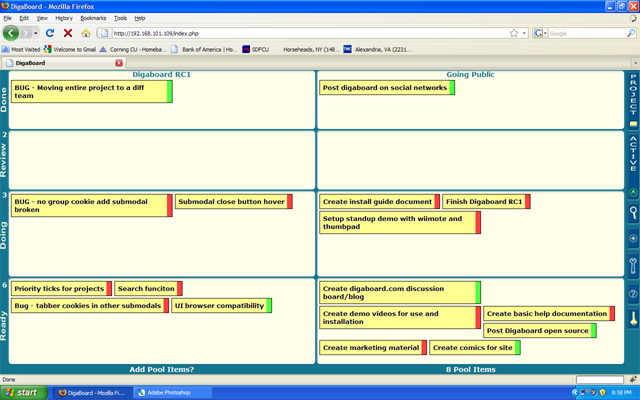
\includegraphics[width=1.0\textwidth]{images/project_board.png}
	\caption{Digaboard Anzeigetafel}
	\label{fig:digaboard}
\end{figure}

Mit dieser Anzeigetafel lassen sich folgende Projektmanagementaufgaben realisieren:
\begin{itemize}
\item Produktanforderungsverwaltung\\
Ein Produkt kann in mehrere Projekte aufgeteilt werden, wobei jedes Projekt seine eigene Spalte in der Anzeigetafel bekommt. Die Anzeigetafel hat mehrere Zeilen, die den Status des Projekts intuitiv darstellen.

\item Task-Planung\\
Die Task-Planung in \emph{Digaboard} ist sehr simpel gehalten. Die Tasks können in der Projekttafel erstellt und einer Zeile zugeordnet werden. Die Zeilen beschreiben den Zustand des Tasks, wie zum Beispiel Ready, Doing, Review und Done. Des Weiteren können hier Fehler eingepflegt werden, die noch zu beseitigen sind.

\item Projektüberwachung\\
Die Projektüberwachung wird durch die übersichtliche Darstellung des Gesamtprozesses auf der Anzeigetafel ermöglicht. Hier können Zeitverzüge bei Tasks leicht erkannt werden.

\item Teamverwaltung\\
Jedes Entwicklerteam bekommt seine eigene Spalte auf der Entwickleranzeigetafel. Dort kann jeder Entwickler seine Taskqueue verwalten.
\end{itemize}

\emph{Digaboard} dient hauptsächlich als Ersatz einer realen Tafel auf der sonst das Projekt dargestellt wird. Diese virtuelle Tafel hat den Vorteil, dass jedes Teammitglied seinen aktuellen Arbeitsstatus über die Webanwendung anpassen kann und sich über den aktuellen Stand des Projektes informieren kann. Jedoch ist die Aufwandsverwaltung und die Zeiterfassung nicht integriert und somit lässt sich \emph{Digaboard} eher als eine Ergänzung für die Projektverwaltung ansehen. \cite {bib:digaboard} \\

\item[IceScrum]\hspace*{1em}\\
Das Projektverwaltungswerkzeug \emph{IceScrum} ist eine web-basierte Server\--Anwendung. Die Anwendung lässt sich mittels eines Webbrowsers ansprechen und benutzen. Der Haupteinsatzzweck dieses Open-Source Werkzeugs ist die agile Vorgehensweise \emph{Scrum}. Zudem bietet \emph{IceScrum} noch Methoden der agilen Vorgehensweise \emph{Kanban}.
Dabei unterstützt die Anwendung das \emph{Scrum} Projektmanagement durch folgende Funktionen:
\begin{itemize}
\item Sprint-Planung\\
Die Sprint-Planung ist bei der agilen Vorgehensweise \emph{Scrum} sehr wichtig. Hierbei können Teammitglieder Tasks für einen Sprint erzeugen. Diese Tasks werden auf einem Dashboard dargestellt. Diese Tasks auf dem Dashboard können dann von Teammitgliedern ausgesucht, begonnen und fertiggestellt werden.

\item Release-Planung\\
Die Planung von Releases erfolgt anhand der Anlegung von Sprints. Innerhalb dieser Sprints werden dann User Stories abgearbeitet. Die Releases werden mit Hilfe der geplanten Sprints und der Teamgröße ermittelt.

\item Produktanforderungsverwaltung\\
Mit Hilfe der Produktanforderungsverwaltung lässt sich die Priorisierung von User Stories durch den Produkt Owner managen.

\item Zeiterfassung\\
Die Zeiterfassung ermöglicht die detaillierte Anzeige von aktuellen Ständen bei Sprints und Releases für jedes Projektmitglied.

\item Projektüberwachung\\
Die Projektüberwachung wird in \emph{IceScrum} durch verschiedene Diagramme wie Burndown, Burnup, Parking Lot und verschiedenen Flussdiagrammen realisiert.

\item Dashboard\\
Das Dashboard ist ein zentraler Bestandteil für den Informationsaustausch. Auf diesem Board sind alle wichtigen Projektinformationen zu finden und auch die letzten Änderungen, Produktvisionen und die Tasks. 
\end{itemize}

Die Entwickler können sich entsprechend ihren Rollen am System einen Account anlegen. So gibt es für jede Projektrolle auch eine dazugehörige Benutzergruppe:
\begin{itemize}
\item Product Owner
\item Scrum Master
\item Stake Holder
\item Developer
\end{itemize}

Des Weiteren bietet \emph{IceScrum} gewisse Funktionen, die aus der \emph{Kanban} Vorgehensweise hervorgehen. Es ist beispielsweise das 'Work in process limit' in die Sprint-Planung mit integriert. \cite{bib:icescrum} \\


\item[XPlanner]\hspace*{1em}\\
Das Open-Source Projekt \emph{XPlanner} hat es sich zur Aufgabe gemacht, die Verwaltung von \emph{XP (Extreme Programming)} Projekten zu unterstützen. \emph{XPlanner} ist ebenfalls ein web-basiertes Werkzeug, dass über einen Webbrowser bedient werden kann. Dabei werden die Methoden des \emph{Extreme Programming} durch folgende Features unterstützt:
\begin{itemize}
\item Planung von User Stories\\
Die Planung von User Stories wird zusammen mit dem Kunden durchgeführt. Der Kunde kann seine gewünschten Funktionalitäten für die nächste Iteration eintragen. Diese Kundenwünsche werden durch den Iteration Manager in Tasks aufgeteilt. Diese Tasks können dann von den Entwicklern in der Iteration abgearbeitet werden.

\item Zeitaufwandserfassung\\
Die Aufwandserfassung ermöglicht den zeitlichen Verlauf von Tasks und User Stories zu ermitteln und auszuwerten. 

\item Entwicklungsprozesse Überwachen\\
Mit \emph{XPlanner} lassen sich sämtliche Tasks, User Stories und Iterationen überwachen. Die Entwicklungsprozesse können nach Status und Zeitablauf visualisiert werden.

\item Task Bearbeitung\\
Die zu bearbeitenden Tasks pro Iteration können von den Entwicklerpaaren ausgewählt werden. 
\end{itemize}

Die Entwickler werden ebenfalls durch eine Zeitaufwandserfassung unterstützt. Diese Zeitaufwandserfassung ermöglicht den Entwicklern eine leichte Aufwandserfassung der geleisteten Arbeit.

Um eine gute Kommunikation mit dem Kunden zu erreichen, hat dieser auch einen Zugang zu dem Projektverwaltungswerkzeug \emph{XPlanner} und kann wie bereits genannt die Funktionen für die nächsten Iterationen vorgeben, die Fortschritte und den Arbeitsaufwand begutachten. Der Kunde kann zusammen mit den Entwicklern einen Release Plan erstellen. \cite{bib:xplanner}

\end{description}

\subsection{Ergebnisse}
Die im vorherigen Punkt vorgestellten Werkzeuge werden nun anhand ihres Funktionsumfanges bewertet. Es wird keine Bewertung in Bezug  auf Usability oder Performance vorgenommen.  Dabei werden die funktionalen Anforderungen für eine Verwaltung aus dem Unterpunkt \ref{ssec:anforderungen} als Betrachtungskriterien herangezogen.

\begin{figure}[h]
  \centering
  \begin{minipage}[c]{0.66\textwidth}
    \begin{tabular}[h]{l|c|c|c|c|c|ccl}
      \textbf{Werkzeuge} & \textbf{ResV} & \textbf{RolV} & \textbf{ ZV } & \textbf{ AV } & \textbf{ PM } & \textbf{ RP }\\
      \hline
      in-Step S. E. & ++ & + & - & ++ & O & ++\\
      TargetProcess & + & ++ & ++ & ++ & + & +\\
      TFS 2010 & ++ & O & + & + & ++ & ++\\
      \hline
      Agilefant & + & ++ & + & + & - & +\\
      Agilo for Scrum & + & ++ & - & - & + & +\\
      Diagboard & - & - - & - & ++ & O & - -\\
      IceScrum & + & ++ & + & + & - - & +\\
      XPlanner & + & ++ & + & + & O & O\\
    \end{tabular}
  \end{minipage}
  \begin{minipage}[c]{0.33\textwidth}
    \begin{tabular}[h]{ll}
      \emph{ResV} & Ressourcenverwaltung\\
      \emph{RolV} & Rollenverteilung\\
      \emph{ZV} & Zeitverwaltung\\
      \emph{AV} & Aufgabenverteilung\\
      \emph{PM} & Problemmanagement\\
      \emph{RP} & Releaseplanung\\
    \end{tabular}
  \end{minipage}
\end{figure}

Die Tabelle zeigt, dass der Funktionsumfang von Open-Source Anwendungen für agile Projektverwaltung zwar denen von proprietären Anwendungen unterlegen ist, jedoch müssen sich die quelloffenen Anwendungen nicht verstecken. Einige Open-Source Projektverwaltungen haben den Umfang, der einen Produktiveinsatz erlaubt. Die proprietären Projektverwaltungssoftwaren können durch eine gute Integration in Entwicklungsumgebungen und in Versionierungssysteme punkten. Desweiteren unterstützen sie die Qualitätssicherung durch die Verwaltung von Tests und die leichte Einpflege von gefundenen Fehlern.

\section{Fazit}
Wie eine Studie von \emph{Forrester Research} zeigt werden agile Vorgehensmodelle bei der Softwareentwicklung zunehmend häufiger eingesetzt und gelten inzwischen als ``Mainstream''. \cite{bib:ane} Als Paradebeispiele für agiles Vorgehen gelten Extreme Programming und Scrum, welche auch zu den beliebtesten Methoden zählen. Sie geben den Entwicklern und Projektbeteiligten wenige klare Regeln an die Hand und steigern dadurch Flexibilität, Effizienz und Transparenz. \cite[S. 28 f.]{bib:wolfRoock} Wenn die Widerstände gegen eine Umstellung auf eine der Methoden zu groß sind, kann die Change-Management-Methode Software Kanban einen sanften Einstieg in die agile Softwareentwicklung zu ermöglichen. Hier wird eine evolutionäre Umstellung der bestehenden Strukturen durchgeführt.

Open Source Projekte harmonieren sehr gut mit einer agilen Softwareentwicklung. Dies zeigen zum Beispiel die Arbeiten an TYPO3 und Firefox. 

Unterstützt werden agile Vorgehensmodelle durch einige Programme. Diese ermöglichen eine transparente Projektplanung und -durchführung. 

\begin{thebibliography}{5}
\bibitem {bib:ane}
Alexander Neumann:
Studie: Agile Softwareentwicklung ist Mainstream.
www.heise.de/-912207, heise online, 25.01.2010, Abgerufen am 21.03.2011

\bibitem {bib:manifest}
Kent Beck, Mike Beedle, Arie van Bennekum, et al.: 
Manifesto for Agile Software Development.
www.agilemanifesto.org, Feb. 2001, Abgerufen am 21.03.2011

\bibitem {bib:eckstein}
Jutta Eckstein: 
Agilität als Geisteshaltung.
www.heise.de/-1188157, heise online, 12.02.2011, Abgerufen am 21.03.2011

\bibitem {bib:wolfRoock}
Henning Wolf, Arne Roock: 
Agile Softwareentwicklung - Ein Überblick.
dpunkt.verlag, 3. Auflage 2011

\bibitem {bib:xp}
James Donovan Wells: 
Extreme Programming - A gentle introduction.
www.extremeprogramming.org, Abgerufen am 28.03.2011

\bibitem {bib:trm}
Mozilla Wiki:
TraceMonkey
\\wiki.mozilla.org/JavaScript:TraceMonkey Abgerufen am 31.3.2011

\bibitem{bib:beltzner}
Mike Beltzner:
Firefox gets more 'Agile' with Lorentz
\\http://www.developer.com/open/article.php/3860226/Mozilla-Firefox-Gets-More-Agile-with-Lorentz.htm Abgerufen am 31.3.2011

\bibitem {bib:gimp}
Golem: Gimp-Entwicklung soll grundlegend verändert werden
http://www.golem.de/1102/81526.html Abgerufen am 31.3.2011

\bibitem {bib:targetprocess}
TargetProcess: Manage any agile project with TargetProcess\\
http://targetprocess.com/Product.aspx

\bibitem {bib:agilefant}
Agilefant: Features\\ 
http://www.agilefant.org/wiki/display/AEF/Features

\bibitem {bib:agilo}
Agilo: The Scrum Tool
http://www.agile42.com/cms/pages/agilo/
http://www.agile42.com/cms/pages/features/

\bibitem {bib:icescrum}
IceScrum: Features\\
http://www.icescrum.org/en/
http://www.icescrum.org/en/features-en/

\bibitem {bib:xplanner}
XPlanner: Homepage\\
http://www.xplanner.org/
http://www.xplanner.org/planning.html

\end{thebibliography}
\end{document}
